\section{peo\-Para\-Pop\-Eval$<$ EOT $>$ Class Template Reference}
\label{classpeo_para_pop_eval}\index{peoParaPopEval@{peoParaPopEval}}
The {\bf peo\-Para\-Pop\-Eval}{\rm (p.\,\pageref{classpeo_para_pop_eval})} represents a wrapper for creating a functor capable of applying in parallel an EO-derived evaluation functor.  


{\tt \#include $<$peo\-Para\-Pop\-Eval.h$>$}

Inheritance diagram for peo\-Para\-Pop\-Eval$<$ EOT $>$::\begin{figure}[H]
\begin{center}
\leavevmode
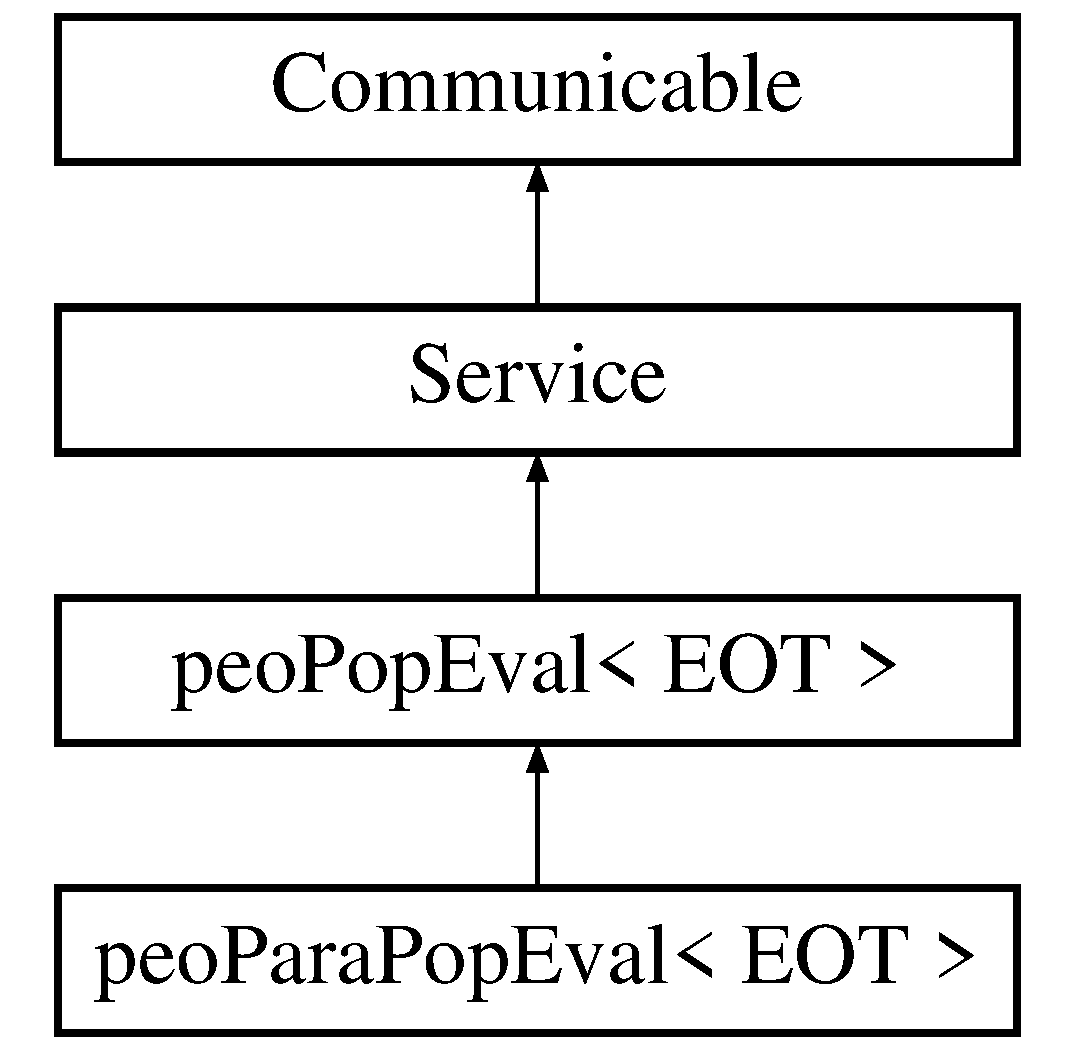
\includegraphics[height=4cm]{classpeo_para_pop_eval}
\end{center}
\end{figure}
\subsection*{Public Member Functions}
\begin{CompactItemize}
\item 
{\bf peo\-Para\-Pop\-Eval} (eo\-Eval\-Func$<$ EOT $>$ \&\_\-\_\-eval\_\-func)
\begin{CompactList}\small\item\em Constructor function - an EO-derived evaluation functor has to be specified; an internal reference is set towards the specified evaluation functor. \item\end{CompactList}\item 
{\bf peo\-Para\-Pop\-Eval} (const std::vector$<$ eo\-Eval\-Func$<$ EOT $>$ $\ast$ $>$ \&\_\-\_\-funcs, {\bf peo\-Agg\-Eval\-Func}$<$ EOT $>$ \&\_\-\_\-merge\_\-eval)
\begin{CompactList}\small\item\em Constructor function - a vector of EO-derived evaluation functors has to be specified as well as an aggregation function. \item\end{CompactList}\item 
void {\bf operator()} (eo\-Pop$<$ EOT $>$ \&\_\-\_\-pop)
\begin{CompactList}\small\item\em Operator for applying the evaluation functor (direct or aggregate) for each individual of the specified population. \item\end{CompactList}\item 
void {\bf pack\-Data} ()
\begin{CompactList}\small\item\em Auxiliary function for transferring data between the process requesting an evaluation operation and the process that performs the actual evaluation phase. \item\end{CompactList}\item 
void {\bf unpack\-Data} ()
\begin{CompactList}\small\item\em Auxiliary function for transferring data between the process requesting an evaluation operation and the process that performs the actual evaluation phase. \item\end{CompactList}\item 
void {\bf execute} ()\label{classpeo_para_pop_eval_3af76378611eac5a36da9a0a00aeeb6c}

\begin{CompactList}\small\item\em Auxiliary function - it calls the specified evaluation functor(s). There is no need to explicitly call the function. \item\end{CompactList}\item 
void {\bf pack\-Result} ()
\begin{CompactList}\small\item\em Auxiliary function for transferring data between the process requesting an evaluation operation and the process that performs the actual evaluation phase. \item\end{CompactList}\item 
void {\bf unpack\-Result} ()
\begin{CompactList}\small\item\em Auxiliary function for transferring data between the process requesting an evaluation operation and the process that performs the actual evaluation phase. \item\end{CompactList}\item 
void {\bf notify\-Sending\-Data} ()
\begin{CompactList}\small\item\em Auxiliary function for notifications between the process requesting an evaluation operation and the processes that performs the actual evaluation phase. \item\end{CompactList}\item 
void {\bf notify\-Sending\-All\-Resource\-Requests} ()
\begin{CompactList}\small\item\em Auxiliary function for notifications between the process requesting an evaluation operation and the processes that performs the actual evaluation phase. \item\end{CompactList}\end{CompactItemize}
\subsection*{Private Attributes}
\begin{CompactItemize}
\item 
const std::vector$<$ eo\-Eval\-Func$<$ EOT $>$ $\ast$ $>$ \& {\bf funcs}\label{classpeo_para_pop_eval_6d69b8f73c0b5d72baf75d6e53f025b7}

\item 
std::vector$<$ eo\-Eval\-Func$<$ EOT $>$ $\ast$ $>$ {\bf one\_\-func}\label{classpeo_para_pop_eval_f0e8af3ee442d2b6baf0bd122226be3c}

\item 
{\bf peo\-Agg\-Eval\-Func}$<$ EOT $>$ \& {\bf merge\_\-eval}\label{classpeo_para_pop_eval_b48bcd4e9f92f364118304535c089456}

\item 
{\bf peo\-No\-Agg\-Eval\-Func}$<$ EOT $>$ {\bf no\_\-merge\_\-eval}\label{classpeo_para_pop_eval_bf255dd5861e27108c2abae7309d7690}

\item 
std::queue$<$ EOT $\ast$ $>$ {\bf tasks}\label{classpeo_para_pop_eval_af76cd18368a0f6185878f37f0b5f272}

\item 
std::map$<$ EOT $\ast$, std::pair$<$ unsigned, unsigned $>$ $>$ {\bf progression}\label{classpeo_para_pop_eval_80e7e34bb1bb2d12f1f2eed3feac6ecf}

\item 
unsigned {\bf num\_\-func}\label{classpeo_para_pop_eval_87abb090c0de39f0ccc36af1f07cca0c}

\item 
EOT {\bf sol}\label{classpeo_para_pop_eval_fb6941e0455515a908eb82342b995163}

\item 
EOT $\ast$ {\bf ad\_\-sol}\label{classpeo_para_pop_eval_60cafeab376262af675fdff43434c8d8}

\item 
unsigned {\bf total}\label{classpeo_para_pop_eval_b528ad9dd9006c3dd57f149a3843e57d}

\end{CompactItemize}


\subsection{Detailed Description}
\subsubsection*{template$<$class EOT$>$ class peo\-Para\-Pop\-Eval$<$ EOT $>$}

The {\bf peo\-Para\-Pop\-Eval}{\rm (p.\,\pageref{classpeo_para_pop_eval})} represents a wrapper for creating a functor capable of applying in parallel an EO-derived evaluation functor. 

The class offers the possibility of chosing between a single-function evaluation and an aggregate evaluation function, including several sub-evalution functions. 



Definition at line 41 of file peo\-Para\-Pop\-Eval.h.

\subsection{Constructor \& Destructor Documentation}
\index{peoParaPopEval@{peo\-Para\-Pop\-Eval}!peoParaPopEval@{peoParaPopEval}}
\index{peoParaPopEval@{peoParaPopEval}!peoParaPopEval@{peo\-Para\-Pop\-Eval}}
\subsubsection{\setlength{\rightskip}{0pt plus 5cm}template$<$class EOT$>$ {\bf peo\-Para\-Pop\-Eval}$<$ EOT $>$::{\bf peo\-Para\-Pop\-Eval} (eo\-Eval\-Func$<$ EOT $>$ \& {\em \_\-\_\-eval\_\-func})}\label{classpeo_para_pop_eval_bcb540510a7038520bec41a7af332daf}


Constructor function - an EO-derived evaluation functor has to be specified; an internal reference is set towards the specified evaluation functor. 

\begin{Desc}
\item[Parameters:]
\begin{description}
\item[{\em eo\-Eval\-Func$<$}]EOT $>$\& \_\-\_\-eval\_\-func - EO-derived evaluation functor to be applied in parallel on each individual of a specified population \end{description}
\end{Desc}


Definition at line 117 of file peo\-Para\-Pop\-Eval.h.

References peo\-Para\-Pop\-Eval$<$ EOT $>$::one\_\-func.\index{peoParaPopEval@{peo\-Para\-Pop\-Eval}!peoParaPopEval@{peoParaPopEval}}
\index{peoParaPopEval@{peoParaPopEval}!peoParaPopEval@{peo\-Para\-Pop\-Eval}}
\subsubsection{\setlength{\rightskip}{0pt plus 5cm}template$<$class EOT$>$ {\bf peo\-Para\-Pop\-Eval}$<$ EOT $>$::{\bf peo\-Para\-Pop\-Eval} (const std::vector$<$ eo\-Eval\-Func$<$ EOT $>$ $\ast$ $>$ \& {\em \_\-\_\-funcs}, {\bf peo\-Agg\-Eval\-Func}$<$ EOT $>$ \& {\em \_\-\_\-merge\_\-eval})}\label{classpeo_para_pop_eval_1cc13a1ec366f95d219d682eccb455bc}


Constructor function - a vector of EO-derived evaluation functors has to be specified as well as an aggregation function. 

\begin{Desc}
\item[Parameters:]
\begin{description}
\item[{\em const}]std :: vector$<$ eo\-Eval\-Func $<$ EOT $>$$\ast$ $>$\& \_\-\_\-funcs - vector of EO-derived partial evaluation functors; \item[{\em peo\-Agg\-Eval\-Func$<$}]EOT $>$\& \_\-\_\-merge\_\-eval - aggregation functor for creating a fitness value out of the partial fitness values. \end{description}
\end{Desc}


Definition at line 126 of file peo\-Para\-Pop\-Eval.h.

\subsection{Member Function Documentation}
\index{peoParaPopEval@{peo\-Para\-Pop\-Eval}!operator()@{operator()}}
\index{operator()@{operator()}!peoParaPopEval@{peo\-Para\-Pop\-Eval}}
\subsubsection{\setlength{\rightskip}{0pt plus 5cm}template$<$class EOT$>$ void {\bf peo\-Para\-Pop\-Eval}$<$ EOT $>$::operator() (eo\-Pop$<$ EOT $>$ \& {\em \_\-\_\-pop})\hspace{0.3cm}{\tt  [virtual]}}\label{classpeo_para_pop_eval_aeaa4fca4f8650e453e308838b4a2cb5}


Operator for applying the evaluation functor (direct or aggregate) for each individual of the specified population. 

\begin{Desc}
\item[Parameters:]
\begin{description}
\item[{\em eo\-Pop$<$}]EOT $>$\& \_\-\_\-pop - population to be evaluated by applying the evaluation functor specified in the constructor. \end{description}
\end{Desc}


Implements {\bf peo\-Pop\-Eval$<$ EOT $>$} {\rm (p.\,\pageref{classpeo_pop_eval_2f208067a5e39c3b26c1234050a41e8f})}.

Definition at line 137 of file peo\-Para\-Pop\-Eval.h.

References peo\-Para\-Pop\-Eval$<$ EOT $>$::funcs, peo\-Para\-Pop\-Eval$<$ EOT $>$::progression, and peo\-Para\-Pop\-Eval$<$ EOT $>$::tasks.\index{peoParaPopEval@{peo\-Para\-Pop\-Eval}!packData@{packData}}
\index{packData@{packData}!peoParaPopEval@{peo\-Para\-Pop\-Eval}}
\subsubsection{\setlength{\rightskip}{0pt plus 5cm}template$<$class EOT$>$ void {\bf peo\-Para\-Pop\-Eval}$<$ EOT $>$::pack\-Data ()\hspace{0.3cm}{\tt  [virtual]}}\label{classpeo_para_pop_eval_fea632bd645ab11182782fd3c038d6d8}


Auxiliary function for transferring data between the process requesting an evaluation operation and the process that performs the actual evaluation phase. 

There is no need to explicitly call the function. 

Reimplemented from {\bf Service} {\rm (p.\,\pageref{class_service_aea4b8f7f8fb88e83862ee4bfd9ab207})}.

Definition at line 158 of file peo\-Para\-Pop\-Eval.h.

References peo\-Para\-Pop\-Eval$<$ EOT $>$::progression, and peo\-Para\-Pop\-Eval$<$ EOT $>$::tasks.\index{peoParaPopEval@{peo\-Para\-Pop\-Eval}!unpackData@{unpackData}}
\index{unpackData@{unpackData}!peoParaPopEval@{peo\-Para\-Pop\-Eval}}
\subsubsection{\setlength{\rightskip}{0pt plus 5cm}template$<$class EOT$>$ void {\bf peo\-Para\-Pop\-Eval}$<$ EOT $>$::unpack\-Data ()\hspace{0.3cm}{\tt  [virtual]}}\label{classpeo_para_pop_eval_410bf4c173e2f36df82251cb16ce1b05}


Auxiliary function for transferring data between the process requesting an evaluation operation and the process that performs the actual evaluation phase. 

There is no need to explicitly call the function. 

Reimplemented from {\bf Service} {\rm (p.\,\pageref{class_service_3bd87b444710813d30fd754d4d0b4df3})}.

Definition at line 172 of file peo\-Para\-Pop\-Eval.h.

References peo\-Para\-Pop\-Eval$<$ EOT $>$::ad\_\-sol, peo\-Para\-Pop\-Eval$<$ EOT $>$::num\_\-func, and peo\-Para\-Pop\-Eval$<$ EOT $>$::sol.\index{peoParaPopEval@{peo\-Para\-Pop\-Eval}!packResult@{packResult}}
\index{packResult@{packResult}!peoParaPopEval@{peo\-Para\-Pop\-Eval}}
\subsubsection{\setlength{\rightskip}{0pt plus 5cm}template$<$class EOT$>$ void {\bf peo\-Para\-Pop\-Eval}$<$ EOT $>$::pack\-Result ()\hspace{0.3cm}{\tt  [virtual]}}\label{classpeo_para_pop_eval_24bb4ae84b0b9f64e7170e3d2b0e1223}


Auxiliary function for transferring data between the process requesting an evaluation operation and the process that performs the actual evaluation phase. 

There is no need to explicitly call the function. 

Reimplemented from {\bf Service} {\rm (p.\,\pageref{class_service_e5e4f90b2315e15c2a2913bd370f4cf5})}.

Definition at line 189 of file peo\-Para\-Pop\-Eval.h.

References peo\-Para\-Pop\-Eval$<$ EOT $>$::ad\_\-sol, and peo\-Para\-Pop\-Eval$<$ EOT $>$::sol.\index{peoParaPopEval@{peo\-Para\-Pop\-Eval}!unpackResult@{unpackResult}}
\index{unpackResult@{unpackResult}!peoParaPopEval@{peo\-Para\-Pop\-Eval}}
\subsubsection{\setlength{\rightskip}{0pt plus 5cm}template$<$class EOT$>$ void {\bf peo\-Para\-Pop\-Eval}$<$ EOT $>$::unpack\-Result ()\hspace{0.3cm}{\tt  [virtual]}}\label{classpeo_para_pop_eval_fd7f0afe9cba30be39269d16097e190e}


Auxiliary function for transferring data between the process requesting an evaluation operation and the process that performs the actual evaluation phase. 

There is no need to explicitly call the function. 

Reimplemented from {\bf Service} {\rm (p.\,\pageref{class_service_45c06344edbfa482b91f68e2035a6099})}.

Definition at line 198 of file peo\-Para\-Pop\-Eval.h.

References peo\-Para\-Pop\-Eval$<$ EOT $>$::ad\_\-sol, Service::get\-Owner(), peo\-Para\-Pop\-Eval$<$ EOT $>$::merge\_\-eval, peo\-Para\-Pop\-Eval$<$ EOT $>$::progression, Communicable::resume(), Thread::set\-Active(), and peo\-Para\-Pop\-Eval$<$ EOT $>$::total.\index{peoParaPopEval@{peo\-Para\-Pop\-Eval}!notifySendingData@{notifySendingData}}
\index{notifySendingData@{notifySendingData}!peoParaPopEval@{peo\-Para\-Pop\-Eval}}
\subsubsection{\setlength{\rightskip}{0pt plus 5cm}template$<$class EOT$>$ void {\bf peo\-Para\-Pop\-Eval}$<$ EOT $>$::notify\-Sending\-Data ()\hspace{0.3cm}{\tt  [virtual]}}\label{classpeo_para_pop_eval_1f78c3cec2940af08a059cc1aa96a9c8}


Auxiliary function for notifications between the process requesting an evaluation operation and the processes that performs the actual evaluation phase. 

There is no need to explicitly call the function. 

Reimplemented from {\bf Service} {\rm (p.\,\pageref{class_service_81ad4d6ebb50045b8977e2ab74826f30})}.

Definition at line 229 of file peo\-Para\-Pop\-Eval.h.\index{peoParaPopEval@{peo\-Para\-Pop\-Eval}!notifySendingAllResourceRequests@{notifySendingAllResourceRequests}}
\index{notifySendingAllResourceRequests@{notifySendingAllResourceRequests}!peoParaPopEval@{peo\-Para\-Pop\-Eval}}
\subsubsection{\setlength{\rightskip}{0pt plus 5cm}template$<$class EOT$>$ void {\bf peo\-Para\-Pop\-Eval}$<$ EOT $>$::notify\-Sending\-All\-Resource\-Requests ()\hspace{0.3cm}{\tt  [virtual]}}\label{classpeo_para_pop_eval_b77031fc4807921ffaf7cf6b669a7665}


Auxiliary function for notifications between the process requesting an evaluation operation and the processes that performs the actual evaluation phase. 

There is no need to explicitly call the function. 

Reimplemented from {\bf Service} {\rm (p.\,\pageref{class_service_f94cc8a5c2665d4574041737e61e9ffc})}.

Definition at line 234 of file peo\-Para\-Pop\-Eval.h.

References Service::get\-Owner(), and Thread::set\-Passive().

The documentation for this class was generated from the following file:\begin{CompactItemize}
\item 
peo\-Para\-Pop\-Eval.h\end{CompactItemize}
